\chapter{Hamiltonian Equation of Motion}
 Hamiltonian method providing a framework for theoretical basis for further developments like Hamiltonian Jacobi theory, perturbation approaches and chaos. Outside classical mechanics Hamiltonian formulation provides much of the language with which present-day statistical mechanics and quantum mechanics is constructed. Throughout the chapter we are assuming mechanical systems are holonomic and the forces are monogenic.
 \begin{itemize}
 	\item In Hamiltonian formulation there can be no constraint equation among the coordinates.
 	\item If $n$ coordinates are not independent, a reduced set of $m$ coordinates, with $m<n$, must be used for the formulation of the problem
 \end{itemize}
\section{Hamiltonian Formulation}
\begin{itemize}
	\item Describe the motion in terms of first order equations of motion
	\item Number of initial conditions determining the motion are stil be $2n$
	\item $2n$ independent first order equations expressed in terms of $2n$ independent variables
	\item $2n$ equations of motion describe behavior of the system point in a phase space
	\item Out of $2n$ independent quantities half of them are $n$ generalized coordinates and other half set to be the generalized or conjugate momenta $p_i$
	\begin{equation}
	  p_i=\frac{\partial L(q_j,\dot{q}_j, t)}{\partial \dot{q}_j}
	\end{equation}
	where $j$ index shows the set of $q$'s and $\dot{q}$'s
	\item The quantities $(p,q)$ are known as the canonical variables
\end{itemize}
\section{Legendre Transformation}
Consider a function of only two variables $f(x,y)$ so that a differential of $f$ has the form
$$df=udx+vdy$$
where
$$u=\frac{\partial f}{dx},\quad v=\frac{\partial f}{dy}$$
To change the basis of description from $x,y$ to a new distinct set of variables $u,y$ so that differential quantities are expressed in terms of $du$ and $dy$
\begin{align*}
\intertext{Let $g$ be a function $u$ and $y$ defined by the equation}
g&=f-ux
\intertext{A differential of $g$ is then given as}
dg&=df-udx-xdu
\intertext{or}
dg&=vdy-xdu
\intertext{and we get}
x=\frac{-\partial g}{\partial u},&\quad v=\frac{\partial g}{\partial y}
\end{align*}
\section{Hamilton Equation of Motion}
Mathematically the transition from Lagrangian to Hamiltonian formulation corresponds to changing the variables in our mechanical functions from $(q, \dot{q}_j,t)$ to $(q,p,t)$ when $p$ is related to $q$ and $\dot{q}$ by
$$p_i=\frac{\partial L(q_j,\dot{q}_j,t)}{\partial \dot{q}_i}$$
The proceedure for switching variables in this manner is provided by the 'Legendre  transformation'.
\begin{align}
\text{Consider Lagrangian }&\ L(q,\dot{q},t)\ \text{ then}\notag\\
dL=\frac{\partial L}{\partial q_i}dq_i&+\frac{\partial L}{\partial \dot{q}_1}+\frac{\partial L}{\partial t}dt\\
\text{The canonical }&\text{momentum  was defined as }p_i=\frac{\partial L}{\partial \dot{q}_i}\notag\\
\text{Substituting it in }&\text{Lagrange equation we obtain}
\dot{p}_i=\frac{\partial L}{\partial {q}_i}\notag\\
\therefore dL&=\dot{p}_idq_i+p_id\dot{q}_i+\frac{\partial L}{\partial t}dt
\intertext{The Hamiltonian $H(q,p,t)$ is generated by the Legendre transformation}
H(q,p,t)&=\dot{q}_ip_i-L(q,\dot{q},t)
\intertext{and has the differential}
dH&=\dot{q}_1dp_i-\dot{p}_1dq_1-\frac{\partial L}{\partial t}dt
\intertext{Where the term $p_id\dot{q}_i$ removed by Legendre transformation since $dH$ can also written as }
dH&=\frac{\partial H}{\partial q_i}dq_1+\frac{\partial H}{\partial p_i}dp_i+\frac{\partial H}{dt}dt
\intertext{We obtain $2n+1$ relations}
&\left.\begin{array}{rl}\dot{q}_{i} & =\frac{\partial H}{\partial p_{i}} \label{HM-07}\\\\ -\dot{p}_{i} & =\frac{\partial H}{\partial q_{i}}\end{array}\right\}\\\notag\\
&-\frac{\partial L}{\partial t}=\frac{\partial H}{\partial t}\notag
\end{align}
Equation $\ref{HM-07}$ are known as the canonical equations of Hamiltonian
\section{Steps to construct Hamiltonian}
Hamiltonian for each problem must be constructed via the Lagrangian formulation.
\begin{enumerate}
	\item With chosen set of generalized coordinates, $q_i$ the Lagrangian $L(\dot{q},\dot{q}_i,t)$=T-V is constructed
	\item The conjugate momenta are defined as function of $q_i,\dot{q}_i$ and $t$ by equation
	$$p_i=\frac{\partial L}{\partial \dot{q}_i}$$
	\item Legendre transformation used to form the Hamiltonian. At this stage we have some mixed functions of $q_i,\dot{q}_i,p_i$ and $t$
	\item $p_i=\frac{\partial L}{\partial \dot{q}_i}$ then converted to obtain $\dot{q}_i$ as functions of $(q,p,t)\ (ie\quad \dot{q}_i=\frac{\partial H}{\partial p_i})$
	\item The result of the previous steps are then applied to eliminate $\dot{q}_i$ from $H$ so to express it solely as a function of $(q,p,t)$
\end{enumerate}
\begin{note}
	In many problems Lagrangian is the sum of functions each homogeneous in the generalized velocities of degree $0,1$ and $2$ respectively in that are
	$$ H=\dot{q}_1p_i-L=\dot{q}_ip-[L_0(q,t)+L_i(q,t)\dot{q}_k+L_1(q_i,t)\dot{q}_k\dot{q}_m]$$
	If equations defining generalized coordinates don't depend on time then $L_2 \dot{q}_k\dot{q}_m=T(K.E)$\\
	If forces are derivable from a consevative potential $V$ (ie work is independent of path), then $L_0=-V$
	When both there conditions are satisfied the Hamiltonian is automatically the total energy
	$$H=T+V=
	E$$
\end{note}
\begin{exercise}
	A particle of inass $m$ moves inside a bowl under gravity. If the surface of the bowl is given by the equation $z=\frac{1}{2} a\left(x^{2}+y^{2}\right)$, where $a$ is a constant.\\
	(A) Write down Lagrangian of the system in cylindrical co-ordinate.\\
	(a) Identified the cyclic coordinate and law of conservation of momentum.\\
	(b) Write down hamiltonion of the system in cylindrical coordinate system.
\end{exercise}
	\begin{answer}
	\begin{align*}
	\text{(A) }T&=\frac{1}{2} m\left(\dot{r}^{2}+r^{2} \dot{\theta}^{2}+\dot{z}^{2}\right)=\frac{m}{2}\left(\dot{r}^{2}+r^{2} \dot{\theta}^{2}+a^{2} r^{2} \dot{r}^{2}\right) \quad \because z=\frac{1}{2} a r^{2} \Rightarrow \quad \dot{z}=a r \dot{r}\\
	V&=m g z=\frac{1}{2} m g a r^{2} \\
	L&=\frac{m}{2}\left[\dot{r}^{2}\left(1+a^{2} r^{2}\right)+r^{2} \dot{\theta}^{2}-a g r^{2}\right]
	\intertext{	(a) $\theta$ is cyclic coordinate}
	\because \frac{\partial L}{\partial \theta}&=0, \Rightarrow \dot{p}_{\theta}=0 \Rightarrow P_{\theta}=\text{ constant}
	\intertext{(b) Hamiltonian}
	H&=\frac{p_{r}^{2}}{2 m\left(1+a^{2} r^{2}\right)}+\frac{p_{\theta}^{2}}{2 m r^{2}}+\frac{1}{2} m a g r^{2} \quad \\&\because \frac{\partial L}{\partial \dot{r}}=p_{r}=m\left(1+a^{2} r^{2}\right) \dot{r}\text{ and }\frac{\partial L}{\partial \dot{\theta}}=p_{\theta}=m r^{2} \dot{\theta}
	\end{align*}
\end{answer}
\begin{exercise}
	A particle of mass $m$ is attached to fixed point $O$ by a weightless inextensible string of length $a$. It is rotating under the gravity as shown in the figure.\\
	(a) Write down The Lagrangian of the system in spherical co-ordinate.\\
	(b) write down Hamiltonian of the system.
	\begin{figure}[H]
		\centering
		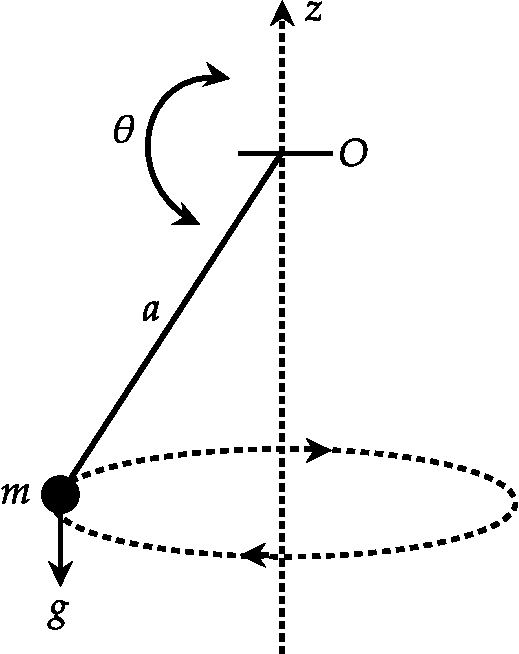
\includegraphics[height=4.5cm,width=3.5cm]{Assignment-HE-02}
	\end{figure}
\end{exercise}
	\begin{answer}
	\begin{align*}
	L&=\frac{1}{2} m\left(\dot{x}^{2}+\dot{y}^{2}+\dot{z}^{2}\right)-[m g(-z)]\\
	L&=\frac{1}{2} m\left(a^{2} \dot{\theta}^{2}+a^{2} \sin ^{2} \theta \dot{\phi}^{2}\right)+m g a \cos (\pi-\theta)\\
	L&=\frac{1}{2} m\left(a^{2} \dot{\theta}^{2}+a^{2} \sin ^{2} \theta \dot{\phi}^{2}\right)-m g a \cos (\theta)\\
	H&=\sum \dot{q}_{1} p_{1}-L\\
	H&=\frac{p_{\theta}^{2}}{2 m a^{2}}+\frac{p_{\phi}^{2}}{2 m a^{2} \sin ^{2} \theta}+m a g \cos \theta \because \frac{\partial L}{\partial \dot{\theta}}=p_{\theta}=m a^{2} \dot{\theta}\text{ and } \frac{\partial L}{\partial \dot{\phi}}=p_{\phi}=m a^{2} \sin ^{2} \theta \dot{\phi}
	\end{align*}
\end{answer}
\begin{exercise}
	Particle of mass $m$ slides under the gravity without friction along the parabotic path
	$y=a x^{2}$ axis shown in the figure. Here $a$ is a constant\\
	(a) Write down Lagrangian of the system .\\
	(b) Write down Lagranges equation of motion.\\
	(c) write down Hamiltonian of the system.
	\begin{figure}[H]
		\centering
		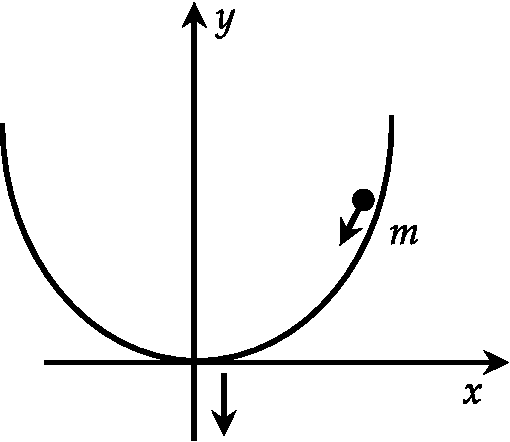
\includegraphics[height=3.5cm,width=4cm]{Assignment-HE-03}
	\end{figure}
\end{exercise}
	\begin{answer}
	\begin{align*}
	y&=a x^{2}\\
	\text{(a) }\dot{y}&=2 a x \dot{x}\\
	L&=\frac{m}{2}\left(\dot{x}^{2}+\dot{y}^{2}\right)-m g y=\frac{m}{2}\left(\dot{x}^{2}+4 a^{2} x^{2} \dot{x}^{2}\right)-m g a x^{2}\\
	L&=\frac{m}{2}\left(1+4 a^{2} x^{2}\right) \dot{x}^{2}-m g a x^{2}\\
	\text{	(b) }&\frac{d}{d t}\left(\frac{\partial L}{\partial \dot{x}}\right)-\frac{\partial L}{\partial x}=0\\
	\frac{d}{d t}&\left[m\left(1+4 a^{2} x^{2}\right) \dot{x}\right]-\left[4 m a^{2} \dot{x}^{2} x-2 \mathrm{~m} g\right.\text{ a }\left.x\right]=0\\
	m \ddot{x}&+4 m a^{2} \ddot{x} x^{2}+8 m a^{2} \dot{x} x \dot{x}-4 m a^{2} \dot{x}^{2} x+2 m g a x=0\\
	m \ddot{x}&+4 m a^{2} x^{2} \ddot{x}+4 m a^{2} x \dot{x}^{2}+2 m g a x=0\\
	\text{(c) }H&=\sum \dot{x} p_{x}-L\\
	H&=\frac{p_{x}^{2}}{2 m\left(1+4 a^{2} x^{2}\right)}+m g a x^{2} \quad \because \frac{\partial L}{\partial \dot{x}}=p_{x}=m\left(1+4 a^{2} x^{2}\right) \dot{x}
	\end{align*}
\end{answer}
\begin{exercise}
	The Lagrangian of a particle of mass $m$ moving in one dimension is $L=\exp (\alpha t)\left[\frac{m \dot{x}^{2}}{2}-\frac{k x^{2}}{2}\right]$, where $\alpha$ and $k$ are positive constants.\\
	(a) Find the Lagranges equation of motion of the particle.\\
	(b) Write down Hamiltonian of the system.
\end{exercise}
	\begin{answer}
	\begin{align*}
	L&=e^{\alpha t}\left(\frac{m \dot{x}^{2}}{2}-\frac{k x^{2}}{2}\right)\\
	\text{(a) }\frac{d}{d t}\left(e^{\alpha t} m \dot{x}\right)-e^{\alpha t} k x&=0 \Rightarrow e^{\alpha t} m \ddot{x}+m \dot{x} e^{\alpha t} \cdot \alpha-e^{\alpha t} k x=0 \Rightarrow e^{\alpha t}[m \ddot{x}+\alpha m \dot{x}-k x]=0\\
	\text{(b) }H&=e^{-\alpha t} \frac{p_{x}^{2}}{2 m}+e^{\alpha t} \frac{k x^{2}}{2}
	\because \frac{\partial L}{\partial \dot{x}}=p_{x}=e^{\alpha t} m \dot{x}
	\end{align*}
\end{answer}
\section{Cyclic Coordinate and Conservation Theorem}
If $q_j$ a cyclic coordinate then, its conjugate momentum $p_j$ is constant.\\
From Lagrangian and Hamiltonian equations of motions:
$$\dot{p}_{j}=\frac{\partial L}{\partial q_{j}}=-\frac{\partial H}{\partial q j}$$
$\therefore$ coordinate that is cyclic will thus also be absent from the Hamiltonian. Conversely if a generalized coordinate does not occur in $H$ the conjugate momentum is conserved.
\begin{itemize}
	\item If $L$ is not explicit function of $t$ then $H$ is a constant of motion 
	\begin{align*}
	\frac{d H}{d t}&=\frac{\partial H}{\partial q_{i}} \dot{q}_{i}+\frac{\partial H}{\partial p_{i}} \dot{p}_{i}+\frac{\partial H}{\partial t}\\\text{substituting }\quad\frac{\partial H}{\partial q_{i}} &=-\dot{p}_{i}\quad\text{ and }\quad\frac{\partial H}{\partial p_{i}} =\dot{q}_{i}\quad\text{we get}\\
	\frac{d H}{d t}&=\frac{\partial H}{\partial t}=\frac{-\partial L}{\partial t}
	\end{align*}
	Therefore if $t$ doesn't appear explicity in $L$, it will also not be present in $H$ and $H$ will be constant in time
	\item If the equations of transformations that define the generalized coordinates
	\begin{equation}
	r_m=r_m(q_1,....q_n,t)\label{HE-02}
	\end{equation}
	do not depend explicity upon the time, and if potantial is velocity independent then $H$ is the total energy $H=T+V$
	\item The identification of $H$ as a constant of motion and as the total energy are two seperate matters. If equation \ref{HE-02} involve time explicity but $H$ doesnot, then $H$ is constant of motion but it is not the total energy.
	\item Unlike $L$, using different set of generalized coordinates in the definition of $H$ may leads to an entirely different quantity for Hamiltonian. It may be that for one set of generalized coordinates $H$ is conserved, but that for another it varies in time.
	\item Explicity first order equations in the $2^{\text{nd}}$ dynamical variables
	\begin{align*}
	\text{If }H&=H(q,p)\text{, ray(autonomous)}\\
	\frac{dH}{dt}&=\frac{\partial H}{\partial q}\dot{q} +\frac{\partial H}{\partial p}\dot{p}\\
	&=\frac{\partial H}{\partial q}\frac{\partial H}{\partial p}-\frac{\partial H}{\partial p}\frac{\partial H}{\partial q}=0\\
	\end{align*}
	Hamiltonian is a constant of motion as long as it is not explicity dependent on time.\\
	Hniltonian governs the time evolution of a system so we call it infinitesimal generator of time translations
\end{itemize}
\section{Other Constants of Motion}
\begin{align*}
\intertext{Suppose $F$ is a constant of motion}
F&=F(q,p,t), \text{it could be explicity time dependent}\\
\frac{dF}{dt}&=\frac{\partial F}{\partial q}\dot{q}+\frac{\partial F}{\partial p}\dot{p}+\frac{\partial F}{\partial t}\\
\frac{dF}{dt}&=\frac{\partial F}{\partial q}\frac{\partial H}{\partial p}-\frac{\partial F}{\partial p}\frac{\partial H}{\partial q}+\frac{\partial F}{\partial t}
\intertext{for $n$ degrees of freedom}
\frac{dF}{dt}&=\sum\limits_{i=1}^{n}\left( \frac{\partial F}{\partial q_i}  \frac{\partial H}{\partial p_i}-\frac{\partial F}{\partial p_i}  \frac{\partial H}{\partial q_i} \right)+\frac{dF}{dt}
\intertext{This constructed out of 2 functions of $F$ and $H$ is called the poisson bracket of $F$ with $H$}
\frac{dF}{dt}&\equiv \underset{poisson bracket}{\left\lbrace F,H\right\rbrace }+ \frac{\partial F}{\partial t}
\end{align*}
It plays the same role in classical mechanics as the commutators of matrices or operators would in quantum mechanics \\
$F$ is a constant of motion if $\frac{dF}{dt}$ vanishes identically\\
$F$= constant of motion if and only if
$$\left\lbrace F,H\right\rbrace +\frac{\partial F}{\partial t}=0$$
it's poisson commute with $H$ or to say $F$ and $H$ are said to be in involution with each other. Where the Hamiltonian itself is a constant of motion for autonomous systems.
\section{Poisson Bracket}
You could define poisson bracket of any two functions of phase variables 
$$\left\lbrace A,B\right\rbrace =\frac{\partial A}{\partial \dot{q}}\ \frac{\partial B}{\partial p}-\frac{\partial A}{\partial p}\ \frac{\partial B}{\partial q}$$
\begin{itemize}
	\item $\left\lbrace A,B\right\rbrace =-\left\lbrace B,A\right\rbrace $ \quad (antisymmetry)\\
	\item $\left\lbrace A+B,C\right\rbrace =\left\lbrace A,C\right\rbrace +\left\lbrace B,C\right\rbrace $
	\item $\left\lbrace \alpha \ A,B\right\rbrace =\alpha\left\lbrace A,B\right\rbrace $
	\item $\left\lbrace A,B C\right\rbrace=B\left\lbrace A,C \right\rbrace+\left\lbrace A,B\right\rbrace C  $ (follow the order)
\end{itemize}
This is the way you could find poisson brackets of various complicated functions of the phase space variable given a few elementary poisson brackets 
$$\left\lbrace A ,\left\lbrace B,C \right\rbrace \right\rbrace +\left\lbrace B ,\left\lbrace C,A \right\rbrace \right\rbrace +\left\lbrace C,\left\lbrace A,B \right\rbrace \right\rbrace =0$$
\section{Conjugate Momentum}
We have independent variable $(q_i...q_N,p_i...p_N)$
\begin{align*}
\left\lbrace q_k,q_l\right\rbrace &=\sum\limits_{i-1}^{n}\left(\frac{\partial q_k}{\partial q_i}\ \frac{\partial q_l}{\partial p_i}-\frac{\partial q_k}{\partial p_i}\ \frac{\partial q_l}{\partial q_i}\right)=0 \text{Since $p$ and $q$ are independent}\\
\left\lbrace p_k,p_l\right\rbrace  &=0  \\
\left\lbrace q_k,p_l\right\rbrace  &=\sum\limits_{i-1}^{n}\left(\frac{\partial q_k}{\partial q_i}\ \frac{\partial p_l}{\partial p_i}-\frac{\partial q_k}{\partial p_i}\ \frac{\partial p_l}{\partial q_i}\right)\\
\left\lbrace q_k,p_l\right\rbrace  &=\sum\limits_{i}\delta_{ik}\delta_{il}=\delta_{kl}
\end{align*}
\textbf{Canonical Poisson Bracket Relations}\\
${q_k,p_l}=\delta_{kl}$\\
${q_k,q_l}=0$\\
${p_k,p_l}=0$\\
once there relations are satisfied\\
momentum $P_K$ is conjugate to the generalized coordinates $q_k (q_k,p_k)$ form conjugate pair\\
for the poisson commutes with all other $p's$ except it's conjugate ${q_k,p_k}=1$
\newpage
\begin{abox}
	Practise set-1
\end{abox}
\begin{enumerate}
	\item A The Hamiltonian of a system with $n$ degrees of freedom is given by $H\left(q_{1}, \ldots . . q_{n} ; p_{1}, \ldots \ldots . p_{n} ; t\right)$, with an explicit dependence on the time $t$. Which of the following is correct?
	{\exyear{	NET/JRF (June-2011) }}
	 \begin{tasks}(1)
		\task[\textbf{a.}]Different phase trajectories cannot intersect each other.
		\task[\textbf{b.}]$H$ always represents the total energy of the system and is a constant of the motion.
		\task[\textbf{c.}]The equations $\dot{q}_{i}=\partial H / \partial p_{i}, \dot{p}_{i}=-\partial H / \partial q_{i}$ are not valid since $H$ has explicit time dependence.
		\task[\textbf{d.}]  Any initial volume element in phase space remains unchanged in magnitude under time evolution.
	\end{tasks}
	\item A If the Lagrangian of a particle moving in one dimensions is given by $L=\frac{\dot{x}^{2}}{2 x}-V(x)$ the Hamiltonian is
	{\exyear{ 	NET/JRF (June-2012)}}
	 \begin{tasks}(2)
		\task[\textbf{a.}]$\frac{1}{2} x p^{2}+V(x)$
		\task[\textbf{b.}]$\frac{\dot{x}^{2}}{2 x}+V(x)$
		\task[\textbf{c.}] $\frac{1}{2} \dot{x}^{2}+V(x)$
		\task[\textbf{d.}] $\frac{p^{2}}{2 x}+V(x)$
	\end{tasks}
	\item B The Hamiltonian of a relativistic particle of rest mass $m$ and momentum $p$ is given by $H=\sqrt{p^{2}+m^{2}}+V(x)$, in units in which the speed of light $c=1$. The corresponding Lagrangian is
	{\exyear{	NET/JRF (DEC-2013)}}
	 \begin{tasks}(2)
		\task[\textbf{a.}]$L=m \sqrt{1+\dot{x}^{2}}-V(x)$
		\task[\textbf{b.}]$L=-m \sqrt{1-\dot{x}^{2}}-V(x)$
		\task[\textbf{c.}]$L=\sqrt{1+m \dot{x}^{2}}-V(x)$
		\task[\textbf{d.}] $L=\frac{1}{2} m \dot{x}^{2}-V(x)$
	\end{tasks}
	\item B A particle of mass $m$ and coordinate $q$ has the Lagrangian $L=\frac{1}{2} m \dot{q}^{2}-\frac{\lambda}{2} q \dot{q}^{2}$, where $\lambda$ is a constant. The Hamiltonian for the system is given by
	{\exyear{ 	NET/JRF (June-2014)}}
	 \begin{tasks}(2)
		\task[\textbf{a.}]$\frac{p^{2}}{2 m}+\frac{\lambda q p^{2}}{2 m^{2}}$
		\task[\textbf{b.}]$\frac{p^{2}}{2(m-\lambda q)}$
		\task[\textbf{c.}] $\frac{p^{2}}{2 m}+\frac{\lambda q p^{2}}{2(m-\lambda q)^{2}}$
		\task[\textbf{d.}] $\frac{p \dot{q}}{2}$
	\end{tasks}
	\item C The Hamiltonian of a one-dimensional system is $H=\frac{x p^{2}}{2 m}+\frac{1}{2} k x$, where $m$ and $k$ are positive constants. The corresponding Euler-Lagrange equation for the system is
	{\exyear{NET/JRF (June-2018)}}
	 \begin{tasks}(2)
		\task[\textbf{a.}] $m \ddot{x}+k=0$
		\task[\textbf{b.}] $m \ddot{x}+2 \dot{x}+k x^{2}=0$
		\task[\textbf{c.}]$2 m x \ddot{x}-m \dot{x}^{2}+k x^{2}=0$
		\task[\textbf{d.}] $m x \ddot{x}+2 m \dot{x}^{2}+k x^{2}=0$
	\end{tasks}
\item D The Hamiltonian of a particle of unit mass moving in the $x y$-plane is given to be: $H=x p_{x}-y p_{y}-\frac{1}{2} x^{2}+\frac{1}{2} y^{2}$ in suitable units. The initial values are given to be $(x(0), y(0))=(1,1)$ and $\left(p_{x}(0), p_{y}(0)\right)=\left(\frac{1}{2},-\frac{1}{2}\right)$. During the motion, the curves traced out by the particles in the $x y$-plane and the $p_{x} p_{y}-$ plane are
{\exyear{ NET/JRF (June-2011)}}
 \begin{tasks}(1)
	\task[\textbf{a.}]Both straight lines
	\task[\textbf{b.}]A straight line and a hyperbola respectively
	\task[\textbf{c.}]A hyperbola and an ellipse, respectively
	\task[\textbf{d.}] Both hyperbolas
\end{tasks}
\item C If the Lagrangian of a dynamical system in two dimensions is $L=\frac{1}{2} m \dot{x}^{2}+m \dot{x} \dot{y}$, then its Hamiltonian is
{\exyear{ NET/JRF (June-2015)}}
 \begin{tasks}(2)
	\task[\textbf{a.}]$H=\frac{1}{m} p_{x} p_{y}+\frac{1}{2 m} p_{y}^{2}$
	\task[\textbf{b.}] $H=\frac{1}{m} p_{x} p_{y}+\frac{1}{2 m} p_{x}^{2}$
	\task[\textbf{c.}]$H=\frac{1}{m} p_{x} p_{y}-\frac{1}{2 m} p_{y}^{2}$
	\task[\textbf{d.}] $H=\frac{1}{m} p_{x} p_{y}-\frac{1}{2 m} p_{x}^{2}$
\end{tasks}
\item A The Hamiltonian of a system with generalized coordinate and momentum $(q, p)$ is $H=p^{2} q^{2} . A$ solution of the Hamiltonian equation of motion is (in the following $A$ and $B$ are constants)
{\exyear{ NET/JRF (June-2016)}}
 \begin{tasks}(2)
	\task[\textbf{a.}] $p=B e^{-2 A t}, \quad q=\frac{A}{B} e^{2 A t}$
	\task[\textbf{b.}] $p=A e^{-2 A t}, \quad q=\frac{A}{B} e^{-2 A t}$
	\task[\textbf{c.}]$p=A e^{A t}, \quad q=\frac{A}{B} e^{-A t}$
	\task[\textbf{d.}] $p=2 A e^{-A^{2} t}, \quad q=\frac{A}{B} e^{A^{2} t}$
\end{tasks}
\item A The Hamiltonian for a system described by the generalised coordinate $x$ and generalised momentum $p$ is
$$
H=\alpha x^{2} p+\frac{p^{2}}{2(1+2 \beta x)}+\frac{1}{2} \omega^{2} x^{2}
$$
where $\alpha, \beta$ and $\omega$ are constants. The corr
{\exyear{NET/JRF (JUNE-2017)}}
 \begin{tasks}(1)
	\task[\textbf{a.}]esponding Lagrangian is
	 $\frac{1}{2}\left(\dot{x}-\alpha x^{2}\right)^{2}(1+2 \beta x)-\frac{1}{2} \omega^{2} x^{2}$
	\task[\textbf{b.}]$\frac{1}{2(1+2 \beta x)} \dot{x}^{2}-\frac{1}{2} \omega^{2} x^{2}-\alpha x^{2} \dot{x}$
	\task[\textbf{c.}]$\frac{1}{2}\left(\dot{x}^{2}-\alpha^{2} x\right)^{2}(1+2 \beta x)-\frac{1}{2} \omega^{2} x^{2}$
	\task[\textbf{d.}] $\frac{1}{2(1+2 \beta x)} \dot{x}^{2}-\frac{1}{2} \omega^{2} x^{2}+\alpha x^{2} \dot{x}$
\end{tasks}
\item C A point mass $m$, is constrained to move on the inner surface of a paraboloid of revolution $x^{2}+y^{2}=a z$ (where $a>0$ is a constant). When it spirals down the surface, under the influence of gravity (along $-z$ direction), the angular speed about the $z$ - axis is proportional to
{\exyear{ NET/JRF (JUNE-2020)}}
 \begin{tasks}(2)
	\task[\textbf{a.}]1 (independent of $z$ )
	\task[\textbf{b.}]$z$
	\task[\textbf{c.}] $z^{-1}$
	\task[\textbf{d.}]  $z^{-2}$
\end{tasks}
\item B The Poisson bracket $\{|\vec{r}|,|\vec{p}|\}$ has the value
{\exyear{ NET/JRF (June-2012)}}
 \begin{tasks}(4)
	\task[\textbf{a.}]$|\vec{r}||\vec{p}|$
	\task[\textbf{b.}]$\hat{r} \cdot \hat{p}$
	\task[\textbf{c.}]3
	\task[\textbf{d.}] 1
\end{tasks}
\item D Let $A, B$ and $C$ be functions of phase space variables (coordinates and momenta of a mechanical system). If ${,}$ represents the Poisson bracket, the value of $\{A,\{B, C\}\}-\{\{A, B\}, C$ is given by
{\exyear{ NET/JRF (DEC-2013)}}
 \begin{tasks}(4)
	\task[\textbf{a.}] 0
	\task[\textbf{b.}]$\{B,\{C, A\}\}$
	\task[\textbf{c.}]$\{A,\{C, B\}\}$
	\task[\textbf{d.}] $\{\{C, A\}, B\}$
\end{tasks}
\item D The coordinates and momenta $x_{i}, p_{i}(i=1,2,3)$ of a particle satisfy the canonical Poisson bracket relations $\left\{x_{i}, p_{j}\right\}=\delta_{i j}$. If $C_{1}=x_{2} p_{3}+x_{3} p_{2}$ and $C_{2}=x_{1} p_{2}-x_{2} p_{1}$ are constants of motion, and if $C_{3}=\left\{C_{1}, C_{2}\right\}=x_{1} p_{3}+x_{3} p_{1}$, then
 \begin{tasks}(1)
	\task[\textbf{a.}]$\left\{C_{2}, C_{3}\right\}=C_{1}$ and $\left\{C_{3}, C_{1}\right\}=C_{2}$
	\task[\textbf{b.}]$\left\{C_{2}, C_{3}\right\}=-C_{1}$ and $\left\{C_{3}, C_{1}\right\}=-C_{2}$
	\task[\textbf{c.}]$\left\{C_{2}, C_{3}\right\}=-C_{1}$ and $\left\{C_{3}, C_{1}\right\}=C_{2}$
	\task[\textbf{d.}] $\left\{C_{2}, C_{3}\right\}=C_{1}$ and $\left\{C_{3}, C_{1}\right\}=-C_{2}$
\end{tasks}
\item A The Hamiltonian of a simple pendulum consisting of a mass $m$ attached to a massless string of length $l$ is $H=\frac{p_{\theta}^{2}}{2 m l^{2}}+m g l(1-\cos \theta)$. If $L$ denotes the Lagrangian, the value of $\frac{d L}{d t}$ is:
{\exyear{ NET/JRF (DEC-2012)}}
 \begin{tasks}(2)
	\task[\textbf{a.}]$-\frac{2 g}{l} p_{\theta} \sin \theta$
	\task[\textbf{b.}] $-\frac{g}{l} p_{\theta} \sin 2 \theta$
	\task[\textbf{c.}]$\frac{g}{l} p_{\theta} \cos \theta$
	\task[\textbf{d.}] $l p_{\theta}^{2} \cos \theta$
\end{tasks}
\item A A particle moves in one dimension in the potential $V=\frac{1}{2} k(t) x^{2}$, where $k(t)$ is a time dependent parameter. Then $\frac{d}{d t}\langle V\rangle$, the rate of change of the expectation value $\langle V\rangle$ of the potential energy is
{\exyear{ NET/JRF (June-2015)}}
 \begin{tasks}(2)
	\task[\textbf{a.}]$\frac{1}{2} \frac{d k}{d t}\left\langle x^{2}\right\rangle+\frac{k}{2 m}\langle x p+p x\rangle$
	\task[\textbf{b.}] $\frac{1}{2} \frac{d k}{d t}\left\langle x^{2}\right\rangle+\frac{1}{2 m}\left\langle p^{2}\right\rangle$
	\task[\textbf{c.}]$\frac{k}{2 m}\langle x p+p x\rangle$
	\task[\textbf{d.}]  $\frac{1}{2} \frac{d k}{d t}\left\langle x^{2}\right\rangle$
\end{tasks}
\item A A particle in two dimensions is in a potential $V(x, y)=x+2 y$. Which of the following (apart from the total energy of the particle) is also a constant of motion?
{\exyear{NET/JRF (DEC-2016)}}
 \begin{tasks}(4)
	\task[\textbf{a.}] $p_{y}-2 p_{x}$
	\task[\textbf{b.}] $p_{x}-2 p_{y}$
	\task[\textbf{c.}]$p_{x}+2 p_{y}$
	\task[\textbf{d.}]  $p_{y}+2 p_{x}$
\end{tasks}
\item A The Hamiltonian of a classical one-dimensional harmonic oscillator is $H=\frac{1}{2}\left(p^{2}+x^{2}\right)$, in suitable units. The total time derivative of the dynamical variable $(p+\sqrt{2} x)$ is
{\exyear{ NET/JRF (JUNE-2018)}}
 \begin{tasks}(4)
	\task[\textbf{a.}]$\sqrt{2} p-x$
	\task[\textbf{b.}] $p-\sqrt{2} x$
	\task[\textbf{c.}]$p+\sqrt{2} x$
	\task[\textbf{d.}]  $x+\sqrt{2} p$
\end{tasks}
\item D A system is governed by the Hamiltonian
$$
H=\frac{1}{2}\left(p_{x}-a y\right)^{2}+\frac{1}{2}\left(p_{x}-b x\right)^{2}
$$
where $a$ and $b$ are constants and $p_{x}, p_{y}$ are momenta conjugate to $x$ and $y$ respectively.
For what values of $a$ and $b$ will the quantities $\left(p_{x}-3 y\right)$ and $\left(p_{y}+2 x\right)$ be conserved?
{\exyear{NET/JRF (June-2013)}}
 \begin{tasks}(2)
	\task[\textbf{a.}]$a=-3, b=2$
	\task[\textbf{b.}]$a=3, b=-2$
	\task[\textbf{c.}]$a=2, b=-3$
	\task[\textbf{d.}] $a=-2, b=3$
\end{tasks}
\item A The Lagrangian of a system moving in three dimensions is
$$
L=\frac{1}{2} m \dot{x}_{1}^{2}+m\left(\dot{x}_{2}^{2}+\dot{x}_{3}^{2}\right)-\frac{1}{2} k x_{1}^{2}-\frac{1}{2} k\left(x_{2}+x_{3}\right)^{2}
$$
The independent constants of motion is/are
{\exyear{NET/JRF (June-2016)}}
 \begin{tasks}(1)
	\task[\textbf{a.}]Energy alone
	\task[\textbf{b.}] Only energy, one component of the linear momentum and one component of the angular momentum
	\task[\textbf{c.}] Only energy, one component of the linear momentum
	\task[\textbf{d.}] Only energy, one component of the angular momentum
\end{tasks}
\item A The Hamiltonian of a system with two degrees of freedom is $H=q_{1} p_{1}-q_{2} p_{2}+a q_{1}^{2}$, where $a>0$ is a constant. The function $q_{1} q_{2}+\lambda p_{1} p_{2}$ is a constant of motion only if $\lambda$ is
{\exyear{NET/JRF (DEC-2019) }}
 \begin{tasks}(2)
	\task[\textbf{a.}]0
	\task[\textbf{b.}]1
	\task[\textbf{c.}]$-a$
	\task[\textbf{d.}]$a$ 
\end{tasks}
\end{enumerate}
 \colorlet{ocre1}{ocre!70!}
\colorlet{ocrel}{ocre!30!}
\setlength\arrayrulewidth{1pt}
\begin{table}[H]
	\centering
	\arrayrulecolor{ocre}
	\begin{tabular}{|p{1.5cm}|p{1.5cm}||p{1.5cm}|p{1.5cm}|}
		\hline
		\multicolumn{4}{|c|}{\textbf{Answer key}}\\\hline\hline
		\rowcolor{ocrel}Q.No.&Answer&Q.No.&Answer\\\hline
		1&\textbf{A} &2&\textbf{A}\\\hline 
		3&\textbf{B} &4&\textbf{B} \\\hline
		5&\textbf{C} &6&\textbf{D} \\\hline
		7&\textbf{C}&8&\textbf{A}\\\hline
		9&\textbf{A}&10&\textbf{C}\\\hline
		11&\textbf{B}&12&\textbf{D}\\\hline
		13&\textbf{D}&14&\textbf{A}\\\hline
		15&\textbf{A}&16&\textbf{A}\\\hline
		17&\textbf{A} &18&\textbf{D}\\\hline
		19&\textbf{A}&20&\textbf{A}\\\hline
		
	\end{tabular}
\end{table}
\newpage
\begin{abox}
	Practise set-2
\end{abox}
\begin{enumerate}
	\item A Consider the Lagrangian $L=a\left(\frac{d x}{d t}\right)^{2}+b\left(\frac{d y}{d t}\right)^{2}+c x y$, where $a, b$ and $c$ are constants. If $p_{x}$ and $p_{y}$ are the momenta conjugate to the coordinates $x$ and $y$ respectively, then the Hamiltonian is
	{\exyear{ 	GATE- 2020}}
	 \begin{tasks}(2)
		\task[\textbf{a.}]$\frac{p_{x}^{2}}{4 a}+\frac{p_{y}^{2}}{4 b}-c x y$
		\task[\textbf{b.}]$\frac{p_{x}^{2}}{2 a}+\frac{p_{y}^{2}}{2 b}-c x y$
		\task[\textbf{c.}]$\frac{p_{x}^{2}}{2 a}+\frac{p_{y}^{2}}{2 b}+c x y$
		\task[\textbf{d.}] $\frac{p_{x}^{2}}{a}+\frac{p_{y}^{2}}{b}+c x y$
	\end{tasks}
	\item A If Hamiltonion is given by $H=\frac{P_{\theta}^{2}}{2 m l^{2}}+m g l(1-\cos \theta)$ Hamilton's equations are then given by
	{\exyear{ 	GATE- 2010}}
	 \begin{tasks}(2)
		\task[\textbf{a.}] $\dot{p}_{\theta}=-m g l \sin \theta ; \quad \dot{\theta}=\frac{p_{\theta}}{m l^{2}}$
		\task[\textbf{b.}]$\dot{p}_{\theta}=m g l \sin \theta ; \quad \dot{\theta}=\frac{p_{\theta}}{m l^{2}}$
		\task[\textbf{c.}]$\dot{p}_{\theta}=-m \ddot{\theta} ; \quad \dot{\theta}=\frac{p_{\theta}}{m}$
		\task[\textbf{d.}] $\dot{p}_{\theta}=-\left(\frac{g}{l}\right) \theta ; \quad \dot{\theta}=\frac{p_{\theta}}{m l}$
	\end{tasks}
	\item B A particle of mass $m$ is attached to a fixed point $O$ by a weightless inextensible string of length $a$. It is rotating under the gravity as shown in the figure. The Lagrangian of the particle is
	$L(\theta, \phi)=\frac{1}{2} m a^{2}\left(\dot{\theta}^{2}+\sin ^{2} \theta \dot{\phi}^{2}\right)-m g a \cos \theta$ where $\theta$ and $\phi$ are the polar angles. The Hamiltonian of the particles is
	{\exyear{ 	GATE- 2012}}
	 \begin{tasks}(2)
		\task[\textbf{a.}]$H=\frac{1}{2 m a^{2}}\left(p_{\theta}^{2}+\frac{p_{\phi}^{2}}{\sin ^{2} \theta}\right)-m g a \cos \theta$
		\task[\textbf{b.}]$H=\frac{1}{2 m a^{2}}\left(p_{\theta}^{2}+\frac{p_{\phi}^{2}}{\sin ^{2} \theta}\right)+m g a \cos \theta$
		\task[\textbf{c.}]$H=\frac{1}{2 m a^{2}}\left(p_{\theta}^{2}+p_{\phi}^{2}\right)-m g a \cos \theta$
		\task[\textbf{d.}] $H=\frac{1}{2 m a^{2}}\left(p_{\theta}^{2}+p_{\phi}^{2}\right)+m g a \cos \theta$
	\end{tasks}
	\item 3 The Hamiltonian for a particle of mass $m$ is $H=\frac{p^{2}}{2 m}+k q t$ where $q$ and $p$ are the generalized coordinate and momentum, respectively, $t$ is time and $k$ is a constant. For the initial condition, $q=0$ and $p=0$ at $t=0, q(t) \propto t^{\alpha}$. The value of $\alpha$ is -----------
	{\exyear{	GATE - 2019 }}
	\item A Consider the Hamiltonian $H(q, p)=\frac{a p^{2} q^{4}}{2}+\frac{\beta}{q^{2}}$, where $\alpha$ and $\beta$ are parameters with appropriate dimensions, and $q$ and $p$ are the generalized coordinate and momentum, respectively. The corresponding Lagrangian $L(q, \dot{q})$ is
{\exyear{	GATE - 2019}}
	 \begin{tasks}(2)
		\task[\textbf{a.}] $\frac{1}{2 \alpha} \frac{\dot{q}^{2}}{q^{4}}-\frac{\beta}{q^{2}}$
		\task[\textbf{b.}]$\frac{1}{2 \alpha} \frac{\dot{q}^{2}}{q^{4}}+\frac{\beta}{q^{2}}$
		\task[\textbf{c.}]$\frac{1}{\alpha} \frac{\dot{q}^{2}}{q^{4}}+\frac{\beta}{q^{2}}$
		\task[\textbf{d.}] $-\frac{1}{2 \alpha} \frac{\dot{q}^{2}}{q^{4}}+\frac{\beta}{q^{2}}$
	\end{tasks}
	\item B The Lagrangian for a particle of mass $m$ at a position $\vec{r}$ moving with a velocity $\vec{v}$ is given by $L=\frac{m}{2} \vec{v}^{2}+C \vec{r} \cdot \vec{v}-V(r)$, where $V(r)$ is a potential and $C$ is a constant. If $\vec{p}_{c}$ is the canonical momentum, then its Hamiltonian is given by
{\exyear{ 	GATE- 2015}}
	 \begin{tasks}(2)
		\task[\textbf{a.}]$\frac{1}{2 m}\left(\vec{p}_{c}+C \vec{r}\right)^{2}+V(r)$
		\task[\textbf{b.}]$\frac{1}{2 m}\left(\vec{p}_{c}-C \vec{r}\right)^{2}+V(r)$
		\task[\textbf{c.}]$\frac{p_{c}^{2}}{2 m}+V(r)$
		\task[\textbf{d.}]  $\frac{1}{2 m} p_{c}^{2}+C^{2} r^{2}+V(r)$
	\end{tasks}
	\item C The Hamiltonian for a system of two particles of masses $m_{1}$ and $m_{2}$ at $\vec{r}_{1}$ and $\vec{r}_{2}$ having velocities $\vec{v}_{1}$ and $\vec{v}_{2}$ is given by $H=\frac{1}{2} m_{1} v_{1}^{2}+\frac{1}{2} m_{2} v_{2}^{2}+\frac{C}{\left(\vec{r}_{1}-\vec{r}_{2}\right)^{2}} \hat{z} \cdot\left(\vec{r}_{1} \times \vec{r}_{2}\right)$, where $C$ is constant. Which one of the following statements is correct?
	{\exyear{GATE- 2015}}
	 \begin{tasks}(1)
		\task[\textbf{a.}] The total energy and total momentum are conserved
		\task[\textbf{b.}]Only the total energy is conserved
		\task[\textbf{c.}]The total energy and the $z$ - component of the total angular momentum are conserved
		\task[\textbf{d.}]  The total energy and total angular momentum are conserved
	\end{tasks}
	\item A The Hamilton's canonical equation of motion in terms of Poisson Brackets are
{\exyear{ 	GATE- 2014}}
	 \begin{tasks}(2)
		\task[\textbf{a.}]$\dot{q}=\{q, H\} ; \dot{p}=\{p, H\}$
		\task[\textbf{b.}]$\dot{q}=\{H, q\} ; \dot{p}=\{H, p\}$
		\task[\textbf{c.}]$\dot{q}=\{H, p\} ; \dot{p}=\{H, p\}$
		\task[\textbf{d.}] $\dot{q}=\{p, H\} ; \dot{p}=\{q, H\}$
	\end{tasks}
	\item B The Poisson bracket $\left[x, x p_{y}+y p_{x}\right]$ is equal to
{\exyear{	GATE- 2017}}
	 \begin{tasks}(4)
		\task[\textbf{a.}] $-x$
		\task[\textbf{b.}]$y$
		\task[\textbf{c.}]$2 p_{x}$
		\task[\textbf{d.}] $p_{y}$
	\end{tasks}
	\item B If $H$ is the Hamiltonian for a free particle with mass $m$, the commutator $[x,[x, H]]$ is
	{\exyear{ GATE - 2018}}
	 \begin{tasks}(4)
		\task[\textbf{a.}]$\hbar^{2} / m$
		\task[\textbf{b.}]$-\hbar^{2} / m$
		\task[\textbf{c.}]$-\hbar^{2} /(2 m)$
		\task[\textbf{d.}] $\hbar^{2} /(2 m)$
	\end{tasks}
	\item B The Poisson bracket between $\theta$ and $\dot{\theta}$ is
{\exyear{	GATE- 2010}}
	 \begin{tasks}(2)
		\task[\textbf{a.}]$\{\theta, \dot{\theta}\}=1$
		\task[\textbf{b.}] $\{\theta, \dot{\theta}\}=\frac{1}{m l^{2}}$
		\task[\textbf{c.}]$\{\theta, \dot{\theta}\}=\frac{1}{m}$
		\task[\textbf{d.}] $\{\theta, \dot{\theta}\}=\frac{g}{l}$
	\end{tasks}
	\item A A dynamical system with two generalized coordinates $q_{1}$ and $q_{2}$ has Lagrangian $L=\dot{q}_{1}^{2}+\dot{q}_{2}^{2}$. If $p_{1}$ and $p_{2}$ are the corresponding generalized momenta, the Hamiltonian is given by
	{\exyear{ JEST-2014}}
	 \begin{tasks}(2)
		\task[\textbf{a.}]$\left(p_{1}^{2}+p_{2}^{2}\right) / 4$
		\task[\textbf{b.}] $\left(\dot{q}_{1}^{2}+\dot{q}_{2}^{2}\right) / 4$
		\task[\textbf{c.}] $\left(p_{1}^{2}+p_{2}^{2}\right) / 2$
		\task[\textbf{d.}]  $\left(p_{1} \dot{q}_{1}+p_{2} \dot{q}_{2}\right) / 4$
	\end{tasks}
\item C The Hamiltonian for a particle of mass $m$ is given by $H=\frac{(p-\alpha q)^{2}}{(2 m)}$, where $\alpha$ is a nonzero constant. Which one of the following equations is correct?
{\exyear{JEST-2020}}
 \begin{tasks}(2)
	\task[\textbf{a.}]$p=m \dot{q}$
	\task[\textbf{b.}]$\alpha \dot{p}=\dot{q}$
	\task[\textbf{c.}] $\ddot{q}=0$
	\task[\textbf{d.}] $L=\frac{1}{2} m \dot{q}^{2}-\alpha q \dot{q}$
\end{tasks}
\item A If the Poisson bracket $\{x, p\}=-1$, then the Poisson bracket $\left\{x^{2}+p, p\right\}$ is ?
{\exyear{JEST-2013}}
 \begin{tasks}(4)
	\task[\textbf{a.}] $-2 x$
	\task[\textbf{b.}]$2 x$
	\task[\textbf{c.}]1
	\task[\textbf{d.}] $-1$
\end{tasks}
\end{enumerate}
 \colorlet{ocre1}{ocre!70!}
\colorlet{ocrel}{ocre!30!}
\setlength\arrayrulewidth{1pt}
\begin{table}[H]
	\centering
	\arrayrulecolor{ocre}
	\begin{tabular}{|p{1.5cm}|p{1.5cm}||p{1.5cm}|p{1.5cm}|}
		\hline
		\multicolumn{4}{|c|}{\textbf{Answer key}}\\\hline\hline
		\rowcolor{ocrel}Q.No.&Answer&Q.No.&Answer\\\hline
		1&\textbf{A} &2&\textbf{A}\\\hline 
		3&\textbf{B} &4&\textbf{3} \\\hline
		5&\textbf{A} &6&\textbf{B} \\\hline
		7&\textbf{C}&8&\textbf{A}\\\hline
		9&\textbf{B}&10&\textbf{B}\\\hline
		11&\textbf{B} &12&\textbf{A}\\\hline
		13&\textbf{C}&14&\textbf{A}\\\hline
	\end{tabular}
\end{table}
\newpage
\begin{abox}
	Practise set-3
\end{abox}
\begin{enumerate}
	\item 	A particle of inass $m$ moves inside a bowl under gravity. If the surface of the bowl is given by the equation $z=\frac{1}{2} a\left(x^{2}+y^{2}\right)$, where $a$ is a constant.\\
	(A) Write down Lagrangian of the system in cylindrical co-ordinate.\\
	(a) Identified the cyclic coordinate and law of conservation of momentum.\\
	(b) Write down hamiltonion of the system in cylindrical coordinate system.
\begin{answer}
	\begin{align*}
	\text{(A) }T&=\frac{1}{2} m\left(\dot{r}^{2}+r^{2} \dot{\theta}^{2}+\dot{z}^{2}\right)=\frac{m}{2}\left(\dot{r}^{2}+r^{2} \dot{\theta}^{2}+a^{2} r^{2} \dot{r}^{2}\right) \quad \because z=\frac{1}{2} a r^{2} \Rightarrow \quad \dot{z}=a r \dot{r}\\
	V&=m g z=\frac{1}{2} m g a r^{2} \\
	L&=\frac{m}{2}\left[\dot{r}^{2}\left(1+a^{2} r^{2}\right)+r^{2} \dot{\theta}^{2}-a g r^{2}\right]
	\intertext{	(a) $\theta$ is cyclic coordinate}
	\because \frac{\partial L}{\partial \theta}&=0, \Rightarrow \dot{p}_{\theta}=0 \Rightarrow P_{\theta}=\text{ constant}
	\intertext{(b) Hamiltonian}
	H&=\frac{p_{r}^{2}}{2 m\left(1+a^{2} r^{2}\right)}+\frac{p_{\theta}^{2}}{2 m r^{2}}+\frac{1}{2} m a g r^{2} \quad \\&\because \frac{\partial L}{\partial \dot{r}}=p_{r}=m\left(1+a^{2} r^{2}\right) \dot{r}\text{ and }\frac{\partial L}{\partial \dot{\theta}}=p_{\theta}=m r^{2} \dot{\theta}
	\end{align*}
\end{answer}
\item 	A particle of mass $m$ is attached to fixed point $O$ by a weightless inextensible string of length $a$. It is rotating under the gravity as shown in the figure.\\
(a) Write down The Lagrangian of the system in spherical co-ordinate.\\
(b) write down Hamiltonian of the system.
\begin{figure}[H]
	\centering
	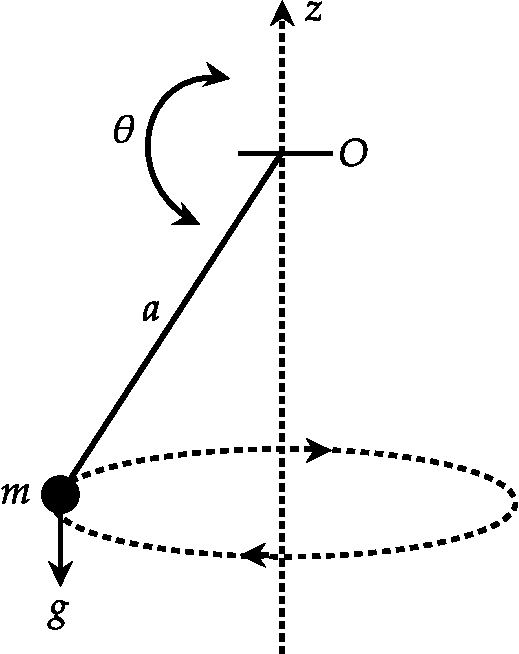
\includegraphics[height=4.5cm,width=3.5cm]{Assignment-HE-02}
\end{figure}
\begin{answer}
\begin{align*}
L&=\frac{1}{2} m\left(\dot{x}^{2}+\dot{y}^{2}+\dot{z}^{2}\right)-[m g(-z)]\\
L&=\frac{1}{2} m\left(a^{2} \dot{\theta}^{2}+a^{2} \sin ^{2} \theta \dot{\phi}^{2}\right)+m g a \cos (\pi-\theta)\\
L&=\frac{1}{2} m\left(a^{2} \dot{\theta}^{2}+a^{2} \sin ^{2} \theta \dot{\phi}^{2}\right)-m g a \cos (\theta)\\
H&=\sum \dot{q}_{1} p_{1}-L\\
H&=\frac{p_{\theta}^{2}}{2 m a^{2}}+\frac{p_{\phi}^{2}}{2 m a^{2} \sin ^{2} \theta}+m a g \cos \theta \because \frac{\partial L}{\partial \dot{\theta}}=p_{\theta}=m a^{2} \dot{\theta}\text{ and } \frac{\partial L}{\partial \dot{\phi}}=p_{\phi}=m a^{2} \sin ^{2} \theta \dot{\phi}
\end{align*}
\end{answer}
\item 	Particle of mass $m$ slides under the gravity without friction along the parabotic path
$y=a x^{2}$ axis shown in the figure. Here $a$ is a constant\\
(a) Write down Lagrangian of the system .\\
(b) Write down Lagranges equation of motion.\\
(c) write down Hamiltonian of the system.
\begin{figure}[H]
	\centering
	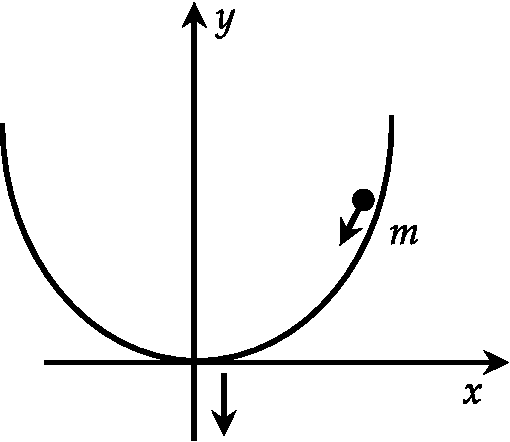
\includegraphics[height=3.5cm,width=4cm]{Assignment-HE-03}
\end{figure}
\begin{answer}$\left. \right. $\\
\begin{align*}
y&=a x^{2}\\
\text{(a) }\dot{y}&=2 a x \dot{x}\\
L&=\frac{m}{2}\left(\dot{x}^{2}+\dot{y}^{2}\right)-m g y=\frac{m}{2}\left(\dot{x}^{2}+4 a^{2} x^{2} \dot{x}^{2}\right)-m g a x^{2}\\
L&=\frac{m}{2}\left(1+4 a^{2} x^{2}\right) \dot{x}^{2}-m g a x^{2}\\
\text{	(b) }&\frac{d}{d t}\left(\frac{\partial L}{\partial \dot{x}}\right)-\frac{\partial L}{\partial x}=0\\
\frac{d}{d t}&\left[m\left(1+4 a^{2} x^{2}\right) \dot{x}\right]-\left[4 m a^{2} \dot{x}^{2} x-2 \mathrm{~m} g\right.\text{ a }\left.x\right]=0\\
m \ddot{x}&+4 m a^{2} \ddot{x} x^{2}+8 m a^{2} \dot{x} x \dot{x}-4 m a^{2} \dot{x}^{2} x+2 m g a x=0\\
m \ddot{x}&+4 m a^{2} x^{2} \ddot{x}+4 m a^{2} x \dot{x}^{2}+2 m g a x=0\\
\text{(c) }H&=\sum \dot{x} p_{x}-L\\
H&=\frac{p_{x}^{2}}{2 m\left(1+4 a^{2} x^{2}\right)}+m g a x^{2} \quad \because \frac{\partial L}{\partial \dot{x}}=p_{x}=m\left(1+4 a^{2} x^{2}\right) \dot{x}
\end{align*}
\end{answer}
\item The Lagrangian of a particle of mass $m$ moving in one dimension is $L=\exp (\alpha t)\left[\frac{m \dot{x}^{2}}{2}-\frac{k x^{2}}{2}\right]$, where $\alpha$ and $k$ are positive constants.\\
(a) Find the Lagranges equation of motion of the particle.\\
(b) Write down Hamiltonian of the system.
\begin{answer}
\begin{align*}
L&=e^{\alpha t}\left(\frac{m \dot{x}^{2}}{2}-\frac{k x^{2}}{2}\right)\\
\text{(a) }\frac{d}{d t}\left(e^{\alpha t} m \dot{x}\right)-e^{\alpha t} k x&=0 \Rightarrow e^{\alpha t} m \ddot{x}+m \dot{x} e^{\alpha t} \cdot \alpha-e^{\alpha t} k x=0 \Rightarrow e^{\alpha t}[m \ddot{x}+\alpha m \dot{x}-k x]=0\\
\text{(b) }H&=e^{-\alpha t} \frac{p_{x}^{2}}{2 m}+e^{\alpha t} \frac{k x^{2}}{2}
\because \frac{\partial L}{\partial \dot{x}}=p_{x}=e^{\alpha t} m \dot{x}
\end{align*}
\end{answer}
\item The Lagrangian of a particle of mass $m$ moving in one dimension is $L=\exp (\alpha t)\left[\frac{m \dot{x}^{2}}{2}-\frac{k x^{2}}{2}\right]$, where $\alpha$ and $k$ are positive constants.\\
(a) Find the Lagranges equation of motion of the particle.\\
(b) Write down Hamiltonian of the system.\\
\begin{answer}
\begin{align*}
L&=e^{\alpha t}\left(\frac{m \dot{x}^{2}}{2}-\frac{k x^{2}}{2}\right)\\
\text{(a) }\frac{d}{d t}\left(e^{\alpha t} m \dot{x}\right)-e^{\alpha t} k x&=0 \Rightarrow e^{\alpha t} m \ddot{x}+m \dot{x} e^{\alpha t} \cdot \alpha-e^{\alpha t} k x=0 \Rightarrow e^{\alpha t}[m \ddot{x}+\alpha m \dot{x}-k x]=0\\
\text{(b) }H&=e^{-\alpha t} \frac{p_{x}^{2}}{2 m}+e^{\alpha t} \frac{k x^{2}}{2}
\because \frac{\partial L}{\partial \dot{x}}=p_{x}=e^{\alpha t} m \dot{x}
\end{align*}
\end{answer}
\item A particle of mass $m$ is attached to fixed point $\mathrm{O}$ by a weightless inextensible string of length $a$. It is rotating under the gravity as shown in the figure.\\
(a) Write down The Lagrangian of the system in spherical co-ordinate.\\
(b) write down Hamiltonian of the system.
\begin{figure}[H]
	\centering
	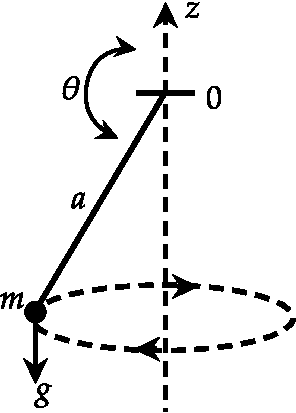
\includegraphics[height=4cm,width=3.5cm]{H-01}
\end{figure}
\item Particle of mass $m$ slides under the gravity without friction along the parabolic path $y=a x^{2}$ axis shown in the figure. Here $a$ is a constant.
(a) write down Lagrangian of the system .
(b) write down Hamiltonian of the system .
\begin{figure}[H]
	\centering
	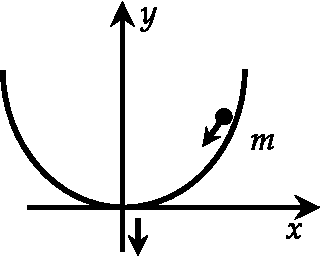
\includegraphics[height=3.5cm,width=4cm]{H-02}
\end{figure}
\item The Lagrangian of a particle of mass $m$ moving in one dimension is $L=\exp (\alpha t)\left[\frac{m \dot{x}^{2}}{2}-\frac{k x^{2}}{2}\right]$, where $\alpha$ and $k$ are positive constants.\\
(a) Write down Hamiltonian of the system.
\item As shown in figure the particle of mass $m_{2}$ moves on a vertical axis and the whole system rotates about this axis with a constant angular velocity $\omega$.\\
(b) Write down Lagrangian of the system in spherical polar co-ordinate.\\
(d) Write down Hamiltonian of the system.
\begin{figure}[H]
	\centering
	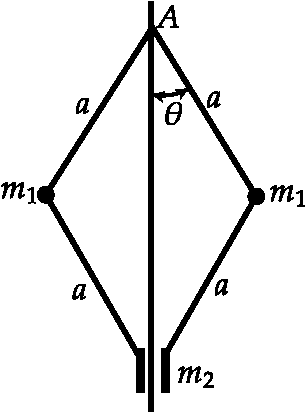
\includegraphics[height=4.5cm,width=3.5cm]{H-03}
\end{figure}
\end{enumerate}